\section{FreePhyloTree y recursos relacionados}
\label{chap:softwares}

\fpt es, actualmente, un visor de la clasificación biológica que, en la
mayoría de los casos, representa un cladograma, aunque no siempre ésto
se cumple, ya que en la clasificación biológica también hay taxones
que son parafiléticos. En un futuro, se espera que la aplicación
visualice árboles filogenéticos, cladogramas, cronogramas y cualquier
tipo de árbol relacionado con la filogenia y la clasificación,
excluyéndo las clasificaciones fenéticas, pues la aplicación siempre
está orientado a estudiar la evolución de las especies\footnote{El
  hecho de incluir en la aplicación información sobre la clasificación
  biológica y no exclusivamente la filogenia, es por un motivo: las
  especies y los grupos evolutivos no se pueden estudiar sino sabes
  como se clasifican, y son dos campos estrechamente unidos,
  \----sobre todo desde que la clasificación se basa en la
  evolución\----}.

\begin{center}
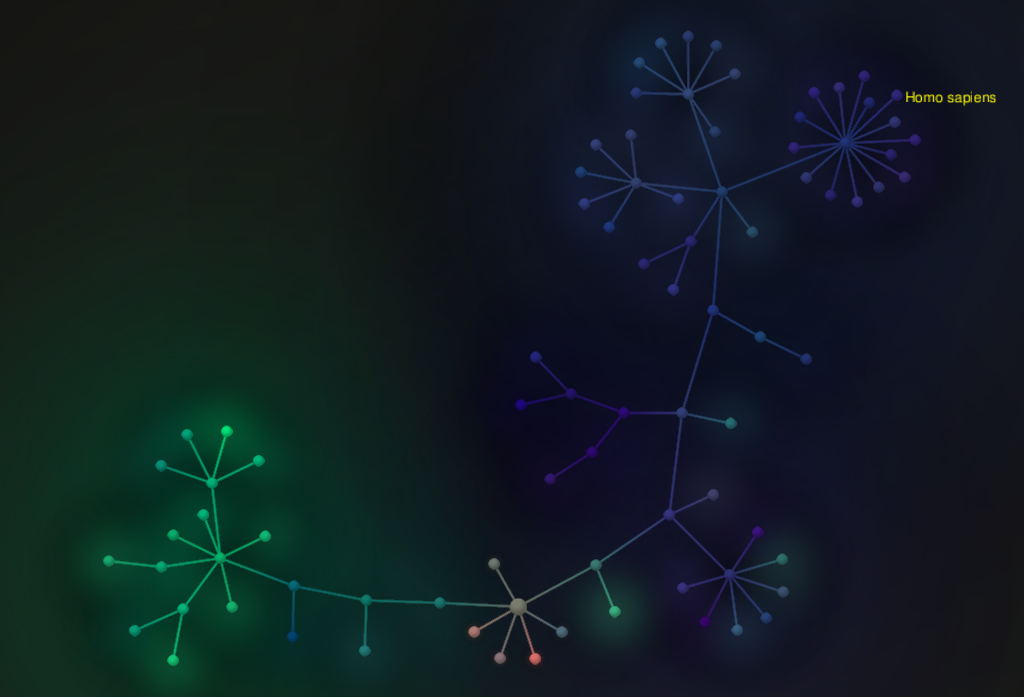
\includegraphics[scale=.5]{../../capture.png}
\end{center}

Ésta es una captura de \fpt. Como vemos, es un árbol que muestra la
clasificación de los primates vista desde el filo
\textit{chordata}, que es la raíz del árbol. La información para
construir el árbol se extrae de \textit{wikispecies}. En la imágen,
\textit{chordata}, se ha expandido dos niveles: se ven sus cuatro
hijos y los hijos de sus hijos. Solo el taxón \textit{vertebrata} se ha
vuelto a expandir. Igualmente, todos los hijos de vertebrata tienen, a
lo sumo, dos niveles de expansión\footnote{El hecho de que sean 2
  niveles es una decisión mía, en compromiso entre la elegancia y
  tiempo de procesamiento, ya que cada expansión requiere una lectura
  al API de \textit{wikispecies}, y a mayor profundidad mayor tiempo
  de lectura, puesto que ésta es recursiva. Con éste equilibrio, el
  usuario nunca tendrá que esperar mucho para que la aplicación
  responda a sus órdenes.}. Nuevamente, el único que hemos vuelto a
expandir ha sido el taxón \textit{tetrapoda}, y así recursivamente
hasta llegar a los primates.

Para terminar de ser una herramienta educativa, hace falta algún
mecanismo de lectura: un texto, documentos o artículos relacionados
con cualquier especie, cualquier concepto o cualquier taxón/clado
presentado, así como mostrar cualquier tipo de información adicional:
como contexto geográfico, climático o temporal. Toda la información
manejada se encapsulará en un wiki, y la aplicación tendrá un
explorador integrado para visualizar los artículos. Sólo con la
lectura puede haber aprendizaje. Para conseguirlo, se ha incrustado un
navegador en la aplicación en la que puede visualizarse el artículo de
\textit{wikipedia} sobre el taxón que deseemos consultar.

Y ésto es todo, lo que por ahora, \fpt hace. Por un lado, puedes
buscar cualquier taxón y ver la clasificación de los subtaxones que
éste contiene, aunque solo en dirección
padre-hijo, pero pronto se podrá explorar la clasificación «hacia
  arriba», es decir, en dirección hijo-padre.

Al lanzar la aplicación, se muestra un menú de ayuda (que puede
ocultarse con F1) con todos los controles existentes, para saber como
expandir o contraer el árbol o como abrir wikipedia.

\subsection{Otros softwares de visualización de taxonomía/filogenia}
Existen otros softwares de visualización de la taxonomía o la
filogenia de las especies, aunque el funcionamiento de éstos softwares
y las bases de datos asociadas participan de todas o algunas de las
siguientes propiedades:

\begin{itemize}
\item El software visualiza árboles filogenéticos a partir de ficheros
  XML. Un fichero XML por árbol filogenético. Éstos ficheros XML
  pueden ser de diversos formatos, y existen estándares \textit{ad
    hoc} sobre el formato de éstos ficheros, que gozan de cierta
  popularidad internacional.
\item Los distintos árboles filogenéticos no se pueden relacionar
  entre sí. Cada fichero es un XML independiente, y no existe ninguna
  base de datos\footnote{Al menos yo no he encontrado ninguna.} que
  contenga una completa clasificación de toda la jerarquía de la
  vida.
\item El software es de corte especializado, y los árboles
  filogenéticos son mostrados o calculados a partir de información
  genética y están diseñadas como herramientas profesionales.
\item Las bases de datos sobre filogenia son sólo de especies vivas,
  ya que para la filogenía de especies fósiles se hace uso exclusivo
  de análisis cladísticos, y éstos análisis no se suman a ninguna base
  de datos global.
\end{itemize}

Existen muchas bases de datos desde distintas universidades u
organismos, pero especializados en ramas concretas o bien necesitan
una licencia para su uso. También existen páginas web, como
\textit{taxonomicon} que almacena información sobre la taxonomía de
muchas especies, mostrando también muchas alternativas según distintos
autores, pero debido a la naturaleza de la página, la información que
allí hay no puede ser usada para montar un software sobre él.

\subsection{Lugares de divulgación relacionados}
\fpt es una herramienta divulgo-educativa, es decir, pretende llegar a
ser una herramienta útil tanto para estudiantes como para
divulgadores. Existen muchos lugares en internet que se dedican a
hacer divulgación científica, desde blogs a wiki, siendo, quizás, la
biología evolutiva la rama más solicitada en divulgación, junto a la
cosmología-astronomía. Como sitios de interés pueden citarse los
siguientes:

\begin{description}
\item[Wikispecies:] Es el wiki usado para construir el árbol de
  \fpt. Ésta página pretende tener actualizada la clasificación más
  moderna y consensuada actualmente, para servir como guía de las
  distintas wikipedias de los distintos idiomas a la hora de crear sus
  correspondientes artículos sobre taxones y/o especies.
\item[Paleofreak:] Blog español sobre paleontología, biología
  evolutiva y temas «afínidos», como el propio autor dice. Es un sitio
  muy visitado y conocido en el mundo de la divulgación científica en
  español, siendo visitado incluso por periodístas, ya que desde ahí
  se hace denuncia de la poca preparación científica de los propios
  periodístas, que suelen publicar noticias llenas de errores
  conceptuales y basadas en prejuicios.
\item[La ciencia y sus demonios:] Otro blog de divulgación donde uno
  de los temas más recurrentes es la biología evolutiva, la
  problemática sobre la religión y la ciencia, etcétera. En algunas
  ocasiones, publican artículos completos dedicados a explicar la
  historia evolutiva de algún grupo biológico en particular.
\item[Palaeos:] Antes sitio web (\textit{palaeos.com}) y ahora wiki
  (\textit{palaeos.org}) basado en la evolución de la vida y de la
  tierra. Sitio web muy interesante con mucha información actualizada
  y excelentes artículos de muchos episodios geológicos y grupos
  biológicos concretos.
\item[Prehistoria universal y vida en la tierra:] Foro en la que se
  abarcan muchos temas, también centrado en biología evolutiva \----aunque
  también hay secciones dedicadas a geología, astronomía,
  etcétera\---- con especial énfasis en la evolución del hombre. Es un
  sitio con poca participación, aunque muchos usuarios y muy
  enriquecido de artículos de muchos temas diversos, del que yo soy
  participante activo y he abierto varios temas, muchos de ellos
  didácticos.
\item[Talkorigins:] Sitio dedicado a discutir sobre el origen
  biológico de las especies o el orígen físico del universo, con un
  carácter ateo-escéptico fuertemente marcado, siendo un lugar también
  muy conocido en el mundo de la divulgación y los debates
  creación-evolución.
\item[Sindioses:] Página de la misma naturaleza que
  \textit{talkorigins} pero en español.
\item[Tree of life web project:] Página web cuyo propósito es mostrar
  la clasificación universal de las especies, y adjuntando artículos
  de cada grupo biológico.
\end{description}

\subsubsection{Propósitos}
Hay muchísimos lugares más, sobre todo blogs, como
\textit{neanderthalensis} o \textit{John Hawks' blog} pero sólo he
resaltado los que considero más importantes y con más repercusión. La
conclusión que hay que sacar es que es un tema con mucho público, hay
muchas personas deseando aprender, y muchas otras deseando enseñar, y
cada página da un enfoque distinto en la medida de sus
posibilidades. \fpt es un intento más de conseguirlo, uniéndo las
ventajas de los softwares y las de la web para suplir las carencias de
uno y otro.

En un futuro, se pretende que la aplicación tenga su propio wiki, con
la información organizada en la forma que \fpt necesita. Es una tarea
titánica hacer de un solo software una herramienta didáctica completa
en éstos campos tan amplios, pero aunando esfuerzos de tanta gente
interesada, y diseñando bien la herramienta de forma que no haya
vacíos que luego los usuarios echen en falta, seguida de publicidad
para que la gente lo conozca, y por último, que guste. La aplicación
se seguirá desarrollando para conseguir todos éstos propósitos y para que
\fpt llege a ser un software de referencia en éstos temas.

También deseo incluir, desde la propia aplicación, un visor gráfico de
toda la información numérica y no exclusivamente textual, como datos
geográficos \----incrustando un mapa y coloreandolo con la
distribución geográfica del grupo en cuestión\----, temporales
\----incrustando una línea temporal y señalando la época en la que
vivió cada grupo\----, la posibilidad de manejar diversas filogenias o
clasificaciones de subárboles, el grado de conversación \----extinto,
en peligro grave de extinción, en peligro leve, etcétera\---- y
cualquier otro tipo de información en forma de datos.
